\section{\textcolor{unibablueI}{Time Table}}
%
\newcommand{\daywidth}{24mm}
\newcommand{\daytextwidth}{21mm}
%
\newcommand{\hourseparation}{3mm}
%
\begin{tikzpicture}[yscale=-0.1, xscale=0.1, node distance=1mm,inner sep = 0pt, outer sep = 0pt]
%
% Style for Days
\tikzstyle{day}=[draw, white, rectangle,  minimum height=5mm, minimum width=\daywidth, fill=unibablueI,anchor=north west, align=center, font=\small]
% Style for hours
\tikzstyle{hour}=[draw, rectangle, minimum height=5mm, minimum width=8mm, fill=unibagrayIV, anchor=north west, align=center, font=\scriptsize]
%
\tikzstyle{default}=[anchor=north west,draw=red]
%
% Styles for events
% Duration of sequences
\tikzstyle{hours}=[rectangle,draw, minimum width=\daywidth, text width=\daytextwidth, anchor=north west, align=center, font=\footnotesize]
\tikzstyle{hhours}=[rectangle,draw, minimum width=.5*\daywidth-1.5mm, text width=.5*\daytextwidth-1.5mm, anchor=north west, align=center, font=\footnotesize]
%
\tikzset{grid/.style={gray,very thin,opacity=1}}
%
%\node[default] at (-7,-12) {
%        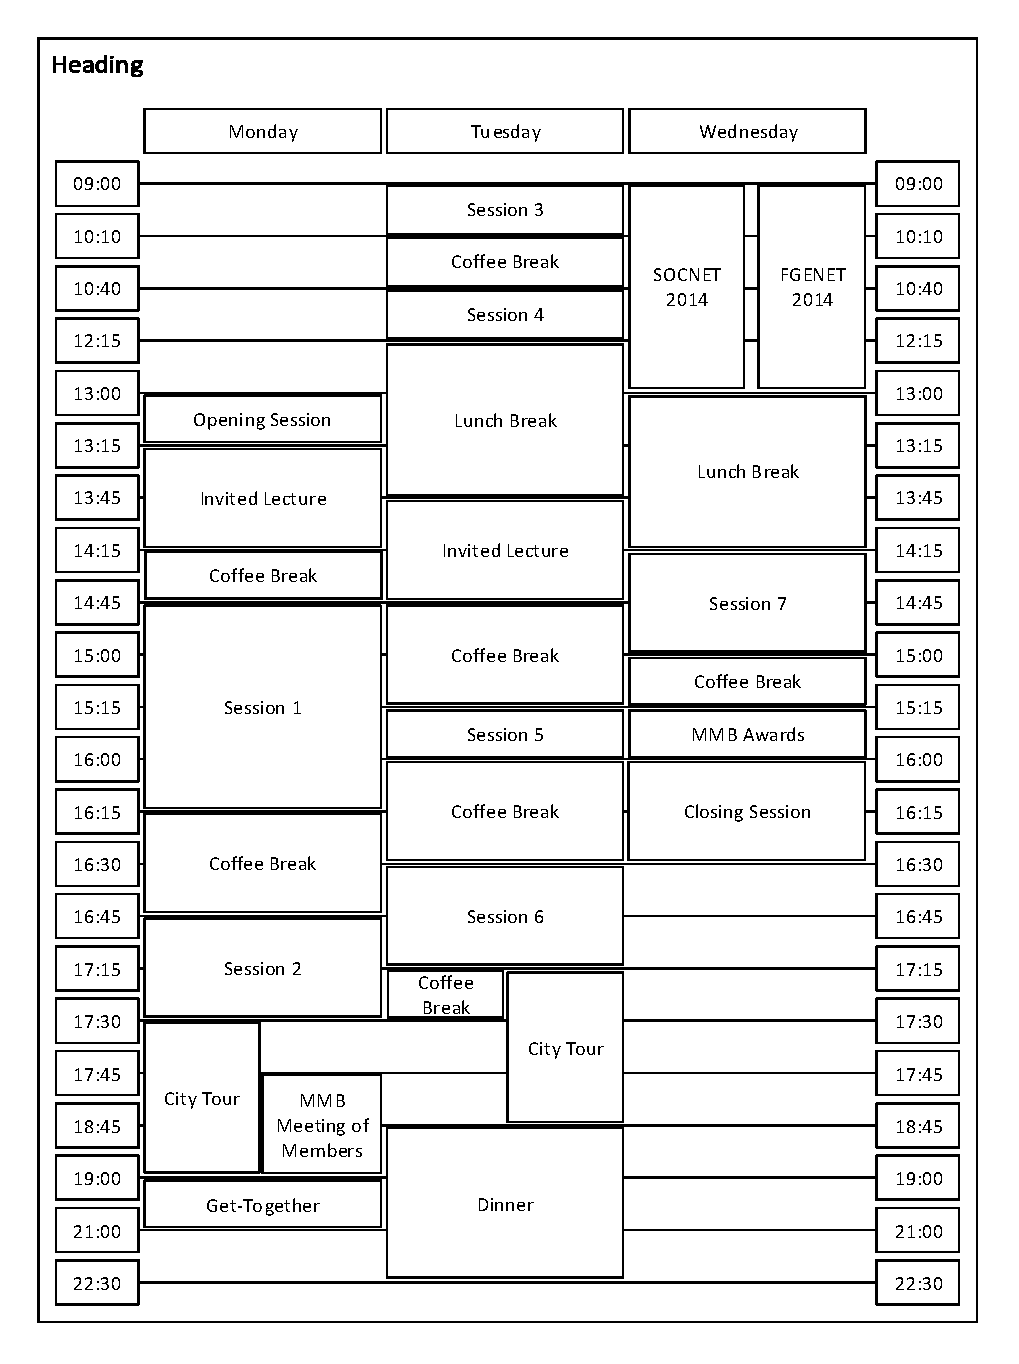
\includegraphics[width=2cm+\textwidth]{images/timetable.pdf}
%    };
%   
%\draw[grid] (0,0) grid (10*\textwidth,10*\textheight);
%
\node[day] (so) at (9,0) {SOCNET};
\node[day] (fg) [right = of so] {FGENET};
\node[day] (wo) [right = of fg] {WoNeCa};
%
\node[hour] (0900) at (0,7) {09:00};
\node[hour] (1000) [below = \hourseparation of 0900] {10:00};
\node[hour] (1025) [below = \hourseparation of 1000] {10:25};
\node[hour] (1125) [below = \hourseparation of 1025] {11:25};
\node[hour] (1145) [below = \hourseparation of 1125] {11:45};
\node[hour] (1150) [below = \hourseparation of 1145] {11:50};
\node[hour] (1210) [below = \hourseparation of 1150] {12:10};
\node[hour] (1310) [below = \hourseparation of 1210] {13:10};
\node[hour] (1315) [below = \hourseparation of 1310] {13:15};
\node[hour] (1600) [below = \hourseparation of 1315] {16:00};

% SOCNET
\node[hours, minimum height = 7mm, fill=unibayellowV] (soil) at($(0900.west)+(so.north west)+(0,.5)$) {\scriptsize Invited Lecture\\ K.A. Zweig};
\node[hours, minimum height = 7mm, fill=white] (socb1) [below = of soil] {Coffee Break};
\node[hours, minimum height = 15mm, fill=unibablueV] (sos1) [below = of socb1] {Session 1};
\node[hours, minimum height = 15mm, fill=white] (socb2) [below = of sos1] {Coffee Break};
\node[hours, minimum height = 7mm, fill=unibablueV] (sos2) [below = of socb2] {Session 2};
\node[hours, minimum height = 7mm, fill=white] (socs) [below = of sos2] {Closing Session};

% FGENET
\node[hours, minimum height = 7mm, fill=unibablueV] (fgs1) at($(0900.west)+(fg.north west)+(0,.5)$) {Session 1};
\node[hours, minimum height = 7mm, fill=white] (fgcb1) [below = of fgs1] {Coffee Break};
\node[hours, minimum height = 7mm, fill=unibayellowV] (fgil) [below = of fgcb1] {\scriptsize Invited Lecture\\ Heddeghem \textit{et al.}};
\node[hours, minimum height = 15mm, fill=white] (fgcb2) [below = of fgil] {Coffee Break};
\node[hours, minimum height = 15mm, fill=unibablueV] (fgs2) [below = of fgcb2] {Session 2};
\node[hours, minimum height = 7mm, fill=white] (fgcs) [below = of fgs2] {Closing Session};

% WoNeCa
\node[hours, minimum height = 71mm, fill=unibagreenV] (so) at($(0900.west)+(wo.north west)+(0,.5)$) {to be announced};

\end{tikzpicture}
\enlargethispage{3ex}